\chapter{Front-end}
\label{cha:front-end}
Per completezza viene riportato un rapido accenno al front-end dell'applicazione, per il quale ho deciso di mantenere lo stesso stile dell'applicativo DISI Industry, per permettere all'utente di avere continuità tra le due applicazioni. Questo capitolo viene presentato per completezza nel documentare tutte le parti dell'applicativo, ma bisogna notare che non è il focus principale, in quanto il progetto è un lavoro di ingegneria del software completo, dall'elicitazione dei requisiti, al design dell'applicativo all'implementazione effettiva della Stack Front-end e Back-end.

Come già citato nella sezione \ref{cha:tecnologie_utilizzate}, sono stati utilizzati Bootstrap ed SCSS per fornire un layout responsive e un design moderno, oltre che a facilitare la stesura di codice CSS. 

\begin{figure}[H]
    \centering
    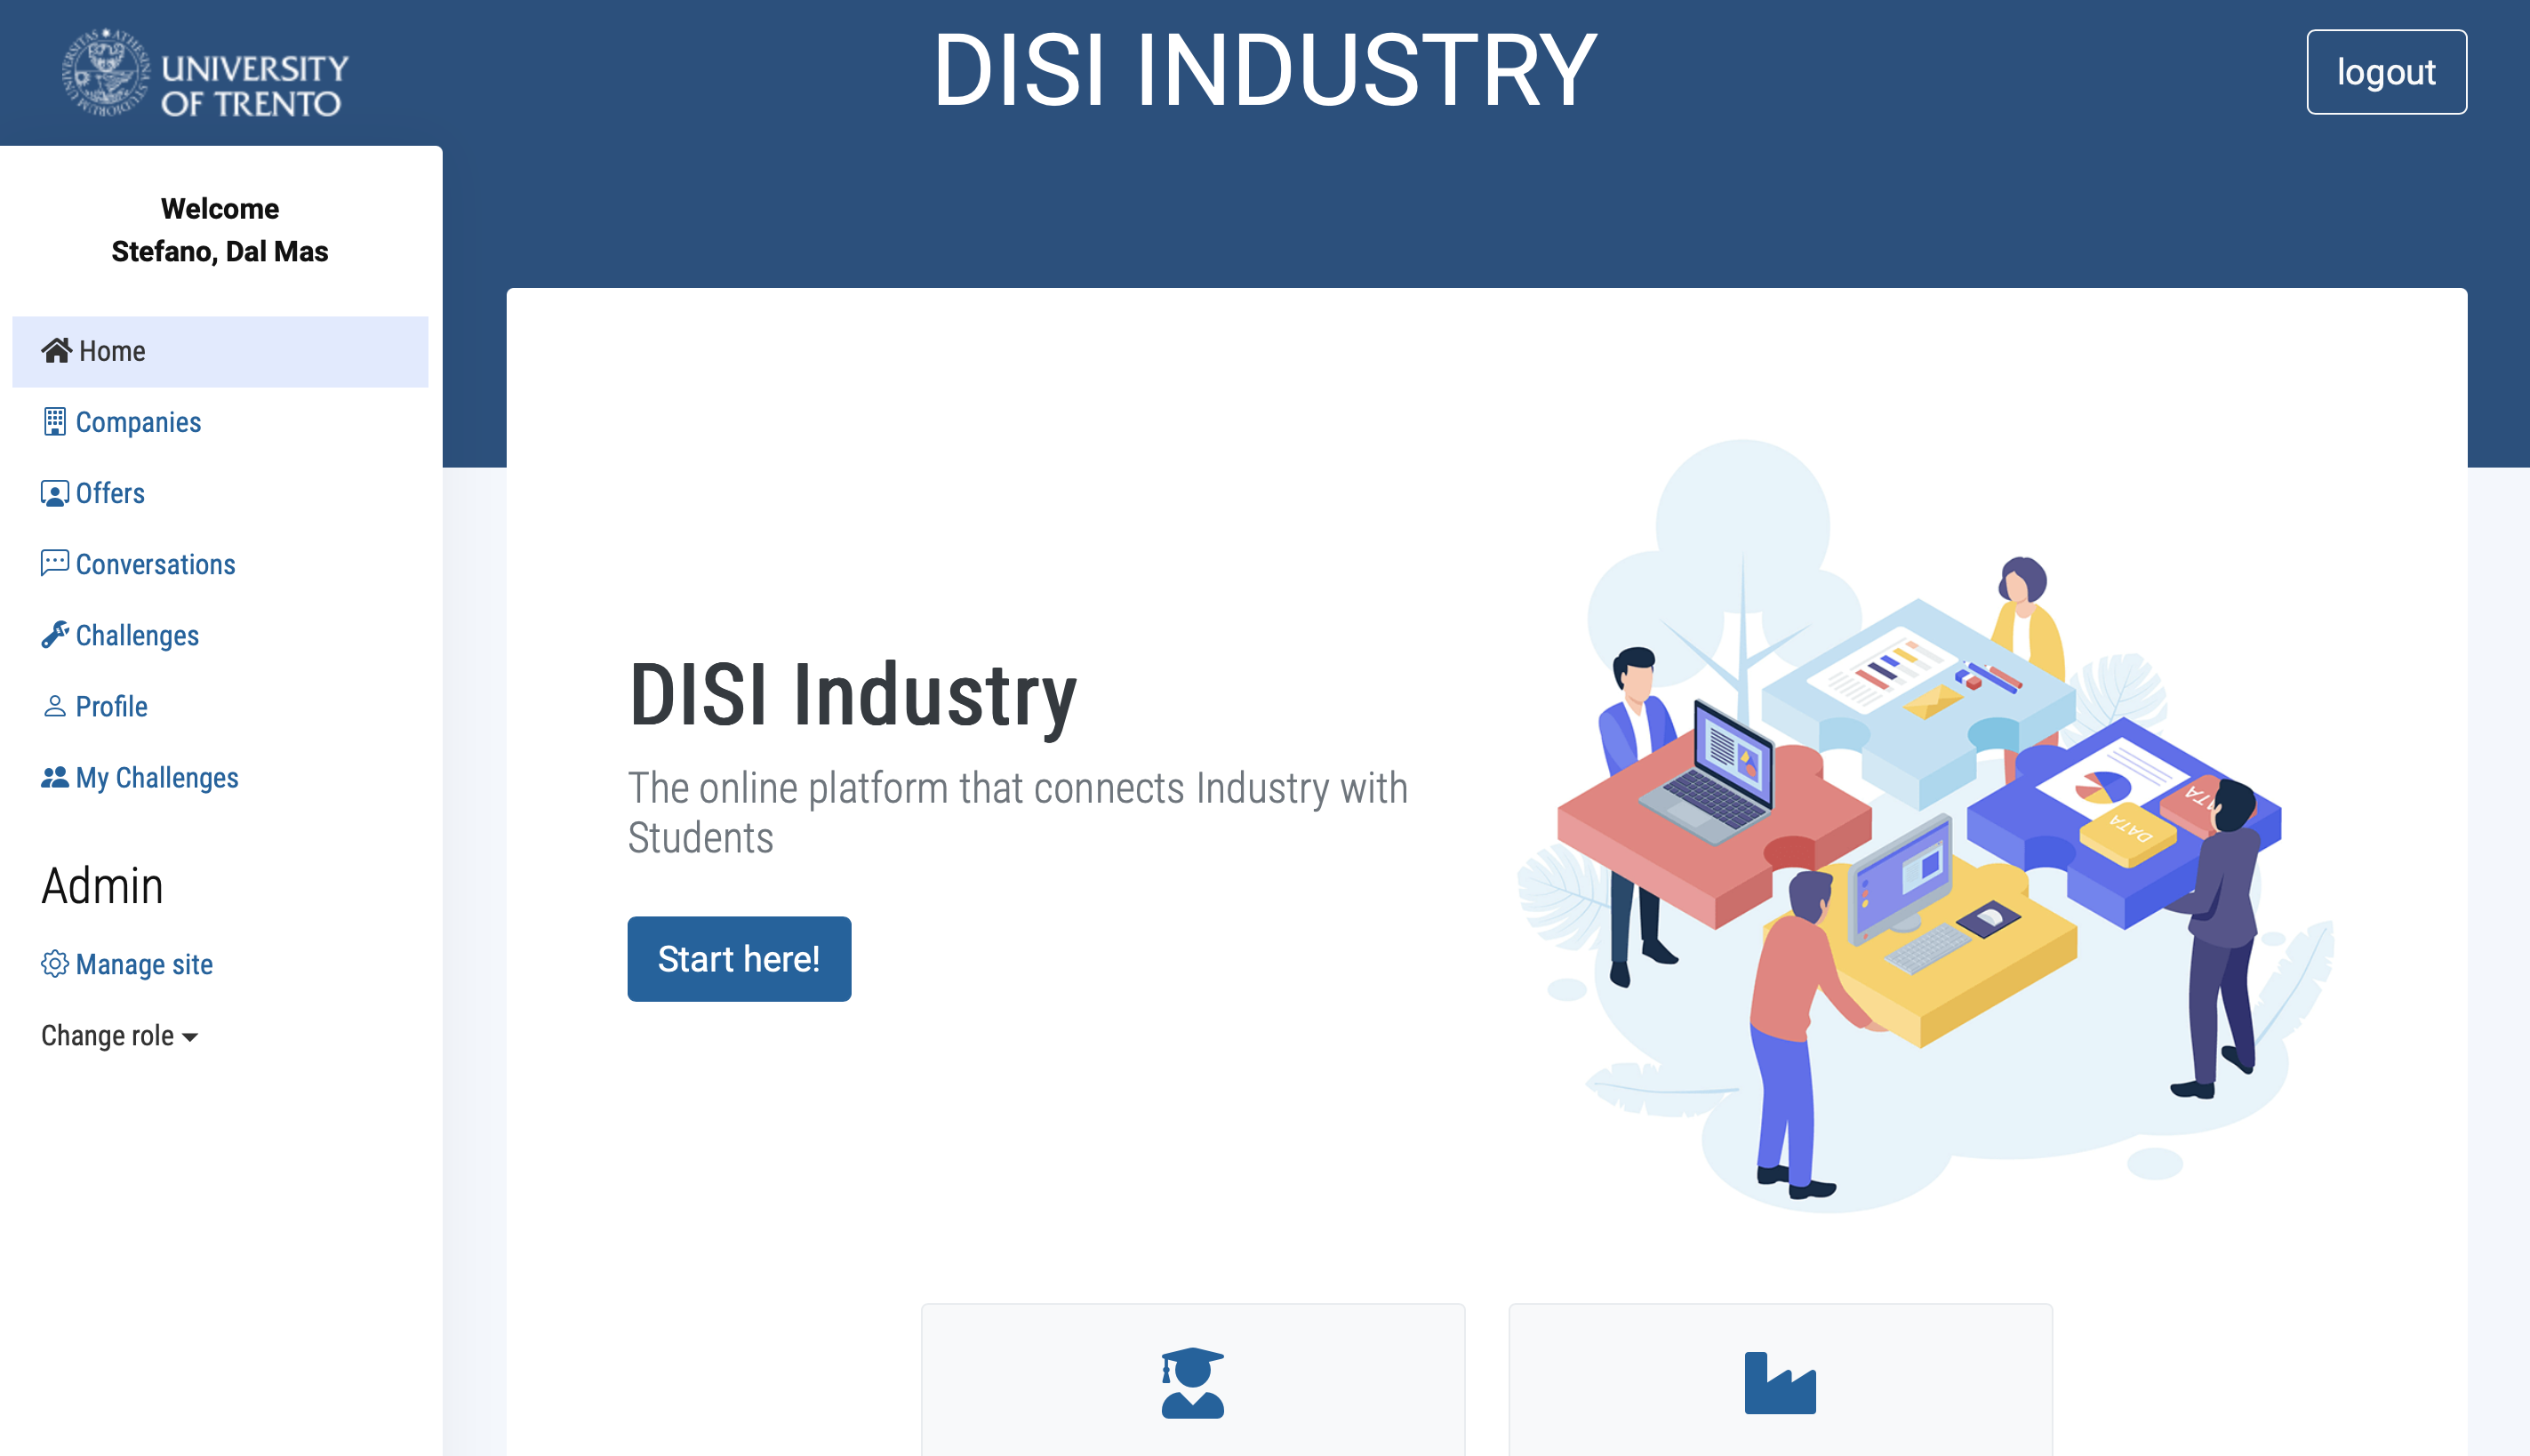
\includegraphics[scale=0.3]{images/home.png}
    \caption{Pagina iniziale dell'applicativo DISI Industry}
    \label{fig:home}
\end{figure}

In questo screenshot viene mostrato lo stile della pagina iniziale di DISI Industry. Tale stile è stato mantenuto per tutta l'applicazione, con piccole modifiche per adattarlo alle nuove funzionalità, senza stavolgerlo per assicurarsi continuità e facilità d'uso per l'utente finale.


Nella sidebar, posta a sinistra della schermata, vi sono varie voci. Dipendentemente dall'attore che sta utilizzando l'applicativo, le voci cambiano per permettere all'utente di accedere in modo semplice alle funzionalità che gli sono disposte.


Di seguito una veloce spiegazione degli utilizzi delle voci dell'applicativo DISI Industry, dal punto di vista dello studente \ref{subsec:studente}
\begin{itemize}
    \item Home : Pagina iniziale di DISI Industry. Spiega il funzionamento ed i vantaggi dell'applicativo.
    \item Companies : permette di visualizzare le compagnie che sono state registrate all'applicativo.
    \item Offers : permette di visualizzare le offerte di stage che sono state pubblicate dalle compagnie.
    \item Conversations : permette di dialogare con le aziende una volta avviata un'offerta con esse.
    \item Manage Site : permette di accedere all'area di moderazione dell'applicativo ed è volta agli utenti che sono Admin.
\end{itemize}

Ovviamente tale voci hanno la funzionalità duale per il Company Manager\ref{subs:company_manager}, ma non vengono riportate in quanto estremamente intuitive da comprendere una volta lette le operazioni a disposizione dello studente.

Durante il lavoro di ampliamento della webapp, sono state inserite delle voci all'interno della sidebar, permettendo all'utente finale di accedere alle nuove funzionalità portate da DISI Challenge. Di seguito vengono riportate tutte le voci aggiunte, con un'indicazione di che attore possa effettuare tali azioni. Per il riferimento agli attori, si veda la sezione \ref{sec:attori} con le relative sottosezioni.


\begin{table}[ht]
    \centering
    \begin{tabularx}{\textwidth}{|c|c|X|}
        \hline
        \textbf{Voce} & \textbf{Attore} & \textbf{Descrizione}\\
        \hline
        Challenges & Company Manager, Studente & Permette di visualizzare le challenge che sono state accettate dal Moderatore \ref{sec:moderatore}. Nel caso del Company Manager, è possibile accedere alla pagina per la creazione di una nuova Challenge. \\
        \hline
        Profile & Student & Permette di selezionare le aree tematiche alle quali lo studente è interessato, oltre a permettere ad esso di selezionare se ricevere o meno mail al momento dell'approvazione di una Challenge da parte del Moderatore.\\
        \hline 
        My Challenges & Student & Permette di visualizzare le Challenge alle quali si è iscritti. Da quella pagina si può accedere al dettaglio del Gruppo di Studenti formato in occasione della Challenge \ref{subsec:gruppo_studenti} ed i relativi dettagli, quali stato del gruppo e valutazioni fornite o ricevute per la Challenge correlata \ref{sec:valutazioni}.\\
        \hline 
        Tutor Area & Tutor & Permette di visualizzare tutti i gruppi che hanno fatto richiesta per tale tutor. Da lì può accedere alla pagina di dettaglio di ogni gruppo e decidere se accettare o meno di partecipare alla Challenge con esso.\\
        \hline
        Manage Laboratories & Moderatore & Permette di visualizzare tutti i laboratori che tale moderatore gestisce. Da lì può accedere alla pagina di dettaglio di ogni laboratorio, visualizzando quindi tutte le Challenge correlate ad esso. Da quest'ultima pagina, può visualizzare il dettaglio della Challenge e decidere se accettarla o meno.\\
        \hline
    \end{tabularx}
    \caption{Tabella delle voci aggiunte dalla WebApp DISI Challenge}
\end{table}

\begin{figure}[H]
    \centering
    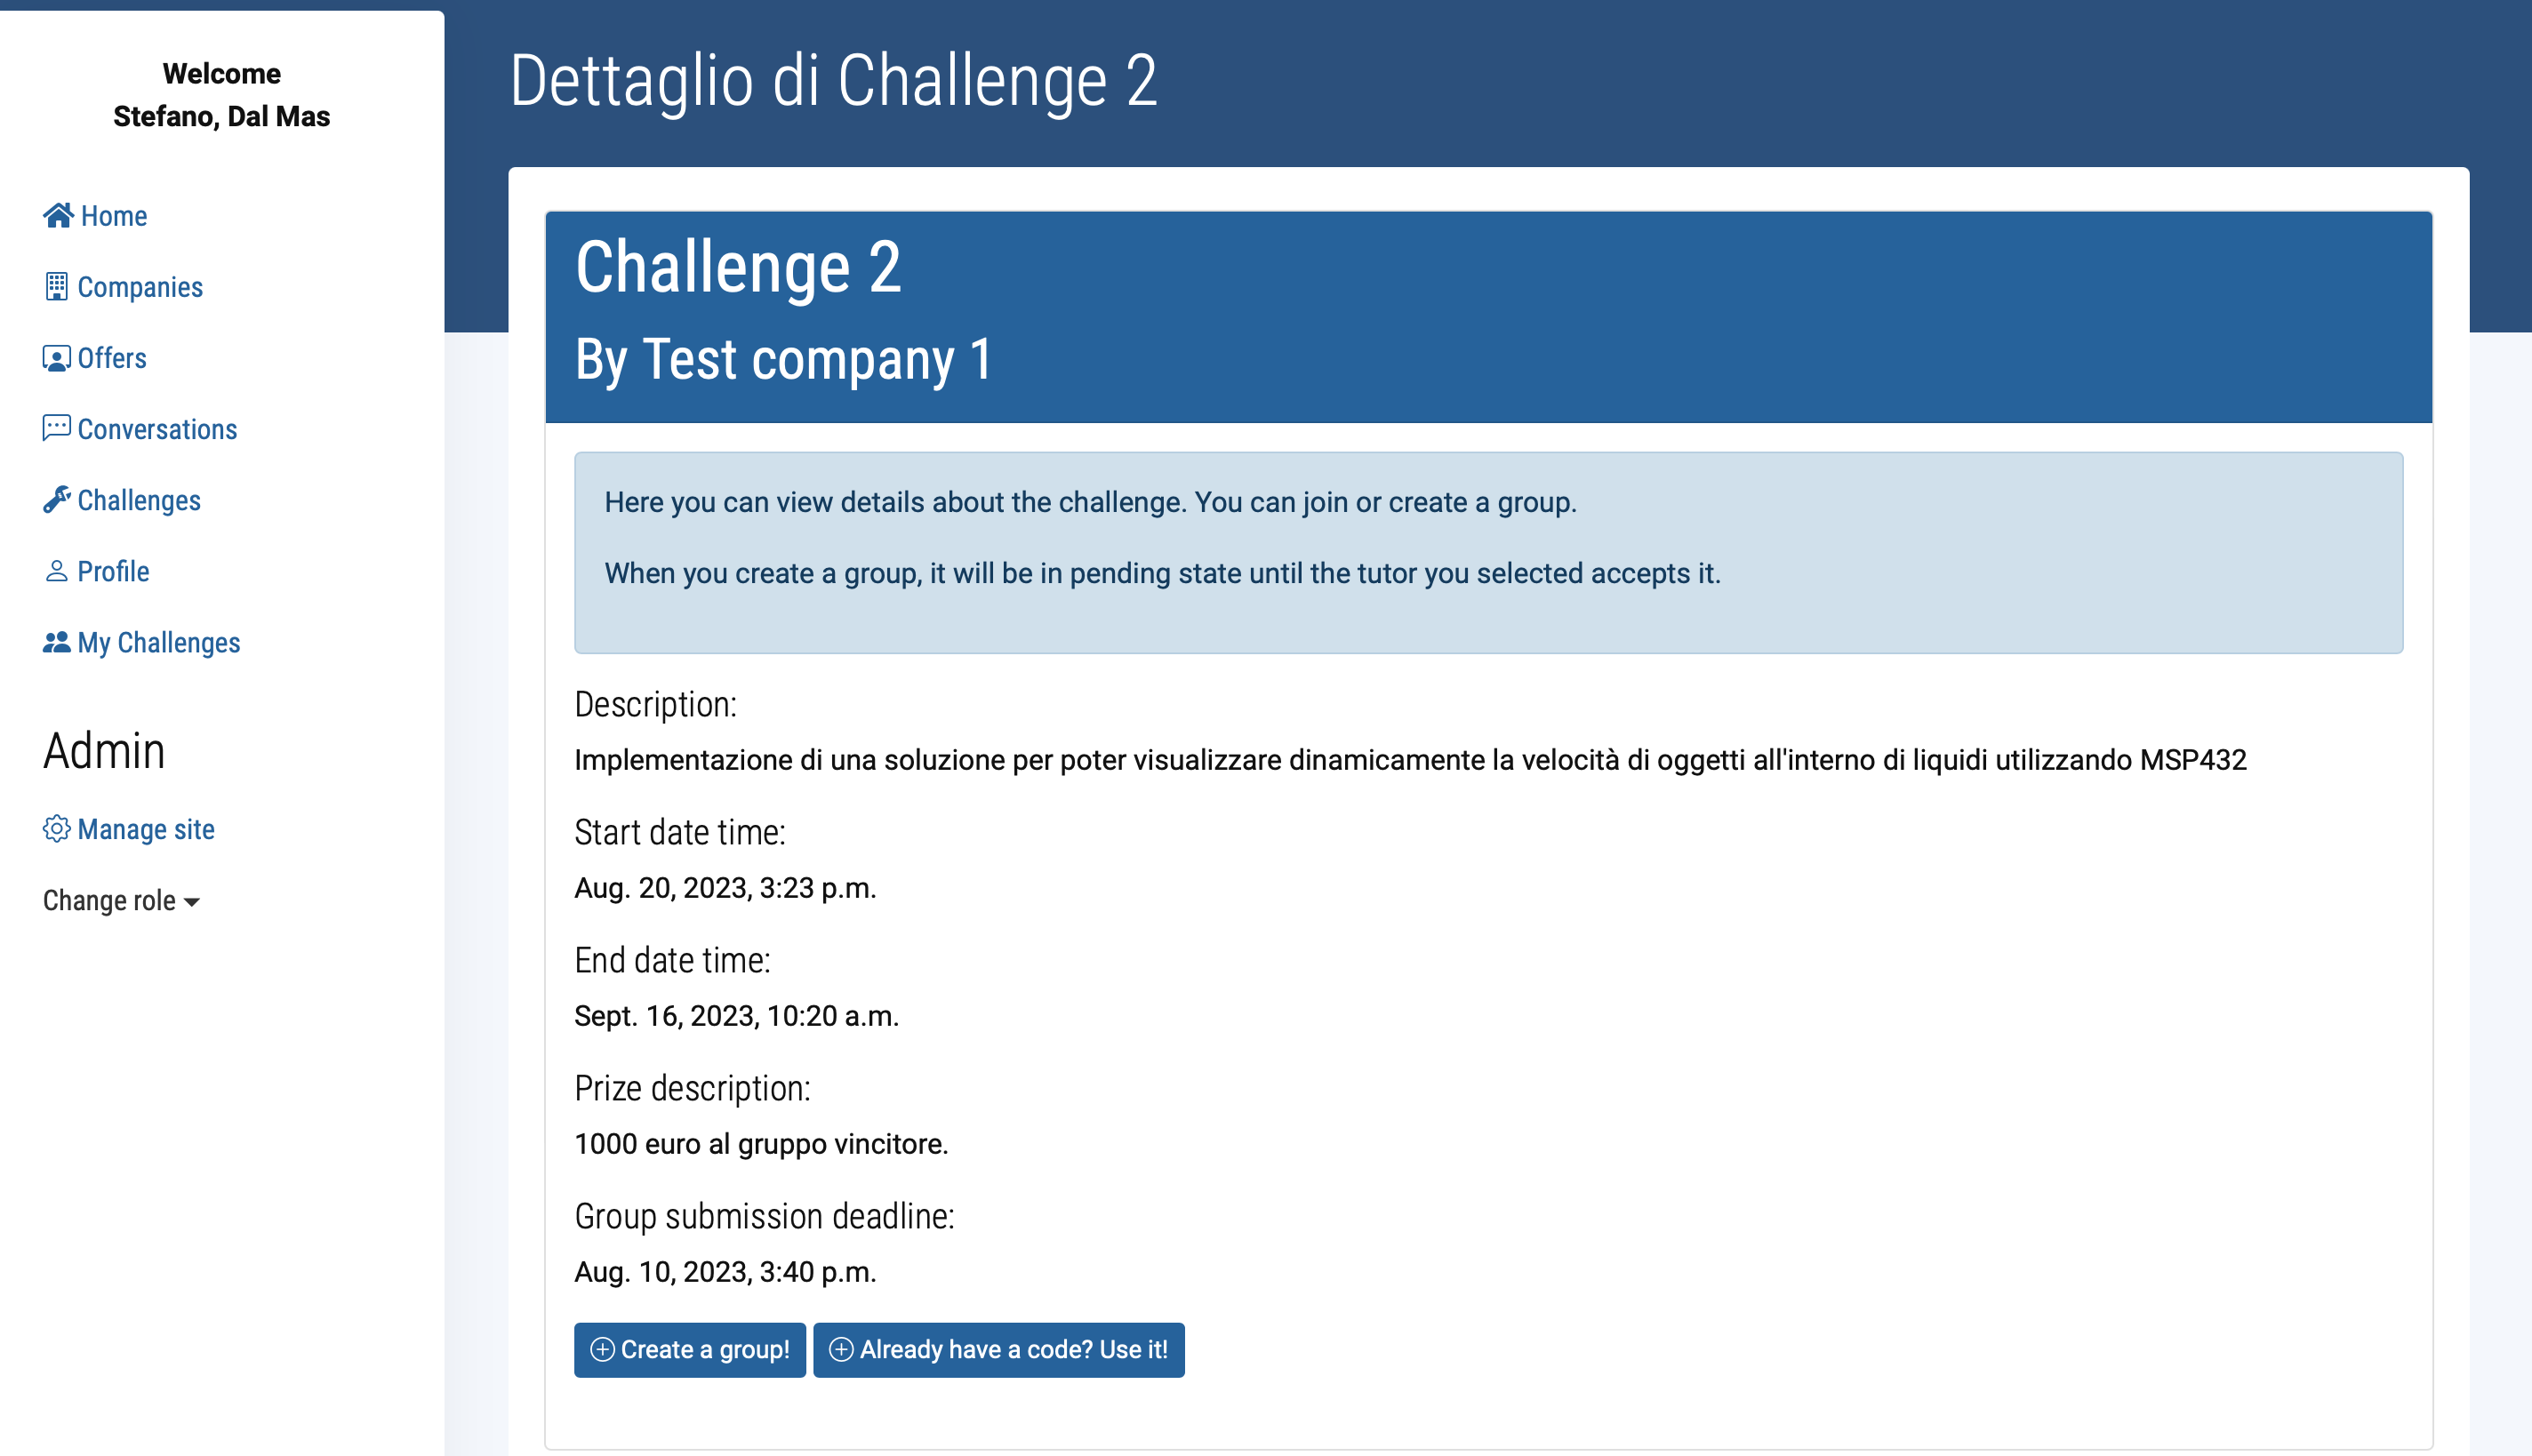
\includegraphics[scale=0.3]{images/challenge_sample.png}
    \caption{Esempio di pagina di dettaglio di una Challenge}
    \label{fig:challenge_sample}
\end{figure}

In questo screenshot, invece, viene rappresentata la pagina di dettaglio di una Challenge, dal punto di vista di uno studente \ref{subsec:studente}.

\clearpage
